\begin{document}
\sectiontitle{9}{Gait Phase Detection}
\setstretch{1.6}

The initial closed loop design involved the use of gait phase detection for use in determining which muscles should be stimulated. The plan was therefore to implement an on-line phase detection algorithm.

\subsection{Methods}
Another student at the lab has decently developed a phase and subphase detection algorithm in python. The plan was therefore to take the newly developed algorithm, adapt it for C++ and implement it in its own thread in Qt. This process was expected to be quite straight forward and was therefore thought to fit within the time frame of the project.

Upon starting the implementation process it however became clear that the algorithm would not be as simple to translate as expected. The issue was that the python implementation used a host of SciPy \cite{noauthor_scipy_nodate} functions in order to implement the algorithm. Scipy is a  widely used library for scientific computing in Python, providing modules for among other things signal processing \cite{noauthor_scipy_nodate}. Unfortunately, no equivalent library, capable of replacing SciPy's functionality exists in C++. After an extensive search for alternatives, it became clear that replicating the necessary SciPy functions would be unavoidable.

\subsection{Implementation}
To implement the gait phase detection, a new class, \texttt{GaitPhaseDetector}, was created to house the custom utility functions and the detection algorithm itself. It proved time consuming and challenging to ensure that the new functions matched the exact functionality of the SciPy functions since the SciPy functions depended on nested calls to other SciPy utilities and the logic could be challenging to interpret. Matching the functionality is hugely important since the entire gait phase and subphase detection algorithm was built and tuned based on the usage of these functions. Despite the challenges, the class was developed and initial results were promising, indicating some degree of success in detecting the peaks needed to then detect the phases of gait as seen in figure \ref{fig:peaks}. 

\begin{figure}
    \centering
    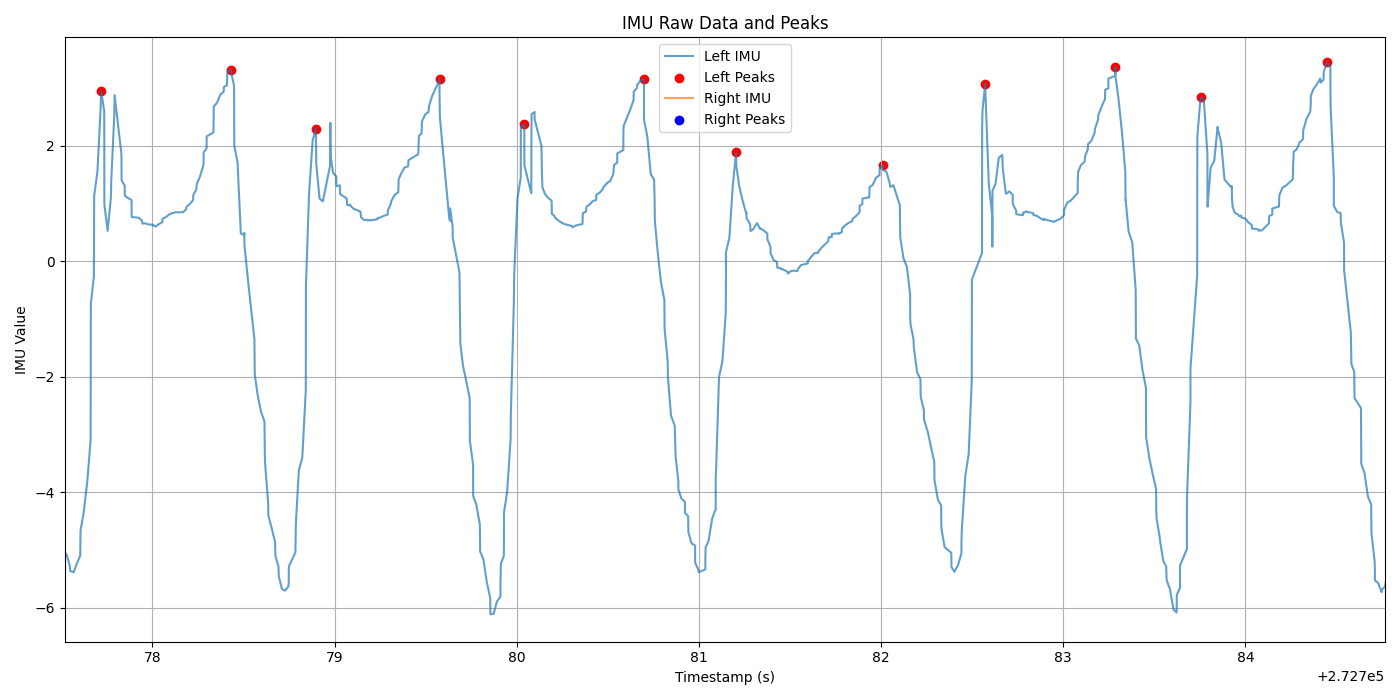
\includegraphics[width=0.95\linewidth]{images/peaks_wz_13.12.24.png}
    \caption{Initial results for peak detection during gait using signal processing functions developed for this project in C++}
    \label{fig:peaks}
\end{figure}

However, upon further testing, it became clear that the results were inconsistent and unreliable. A possible contributing factor here might be the potential discrepancies in the implementation of the SciPy functions. Despite thorough efforts to accurately replicate the functionality, subtle differences likely persisted which can have impacted the algorithm's performance. 

Another major challenge was the need to retune some of the algorithm parameters. The detection algorithm has been meticulously tuned throughout months of work to achieve a reliable and generalizable gait phase detector. The parameters include thresholds for metrics such as peak widths, which were defined as the number of data entries on either side of a peak. This posed  a significant challenge during adaptation since even when the C++ implementation exactly replecated the method in which data aquisition was managed in the Python implementation ( stream inlet in while loop) the frequency of incoming data differed. This discrepancy necessitates the retuning of all parameters that rely on counting the number of data points. This is a time consuming process. 

\subsection{Results}
While the adaptation of the Python-based gait phase detection algorithm to C++ initially appeared feasible within the project
s timeframe, the complexity of replicating SciPy's functionality and retuning the algorithm's parameters introduces significant challenges leading to the conclusion that implementing on-line gait phase detection would not be feasible within the time-frame of the project. However the initial implementation of the GaitPhaseDetector class is implemented with the architecture and stands ready to be more further developed and finished by later students.


\end{document}